%% Bachelor Thesis Template of Xidian Uniersity
%%   for using XDBAthesis package with LaTeX
%%
%% Created by Xue-Jilong(xuejilong@gmail.com)
%%
%% template.tex v0.1, 2011/03/21


\documentclass[xetex]{XDBAthesis}
% 选项说明:
% dvipdfm  使用 dvipdfm(x) 生成最终的 PDF 文档 (缺省设置)
% dvips    使用 dvips 生成最终的 PS 文档
% pdftex   使用 pdfLaTeX 生成最终的 PDF 文档
% xetex    使用 XeLaTeX 生成 PD F文档
% adobefonts 使用 Adobe 中文字体
% winfonts 使用 Windows 中文字体
% master   用于生成硕士学位论文


% 图形文件的搜索路径
\graphicspath{{chapter/Images/}{figures/}}

\begin{document}

%%----------------- 封面部分 ----------------- %%
    \class{3-0891}
    \schoolnumber{03089001}
%    \title{面向数据查询的MapReduce框架}{设计与实现}   %%题目超过14个字把剩下的放到第二个空
	\title{基于Hadoop的MapReduce程序设计}{开发及性能研究}
    \college{计算机学院}
    \major{计算机科学与技术}
    \author{张易}
    \advisor{崔江涛}
    \maketitle

%%----------------- 前言部分 ----------------- %%
    \frontmatter
    \begin{abstract}
在计算机历史上,每一次技术的进化都伴随着数据的爆炸,这些海量增长的数据日益成为人们所关注的焦点。在计算机行业内,如何高效快速的处理这些海量数据,一直是学术界所热议的话题。

MapReduce是Google公司在2004年在OSDI国际会议上提出的一种简单的并行计算模型,它借鉴了函数式编程语言的特点,将大规模数据的分布式处理程序抽象为一个运行在分布式集群上的Map函数和Reduce函数,从而实现了分布式处理海量数据。Hadoop是MapReduce的开源实现。

本文基于Hadoop平台,针对Hadoop的两种运行机制设计并开发出了Web访问日志处理程序,并通过一定的测试将Hadoop两种运行机制的性能做以对比,继而找出Hadoop现有不足。

\keywords{MapReduce   Hadoop   开发   性能}
\end{abstract}

\begin{englishabstract}
Every evolution in the computer's history comes with the explosion of data. People has shown a lot of interests to the massive growth of data. How to process these data rapidly and efficiently has been a hot topic by the academics. 

MapReduce is a simple programing framework published by Google Company in 2004 in OSDI International Conference. It draws on the characteristics of functional programming languages​​ and abstracts a large-scale distributed data handler as a pair of Map and Reduce functions which run in a distributed cluster to process huge amounts of data. Hadoop is an open source implementation of MapReduce.

This thesis based on Hadoop platform. Aim to develop a software, which can process the access logs generated by webserver, in two different ways provided by Hadoop and compare the performance of these two methods then found the insignificancy of Hadoop platform.

\englishkeywords{MapReduce   Hadoop   Programing   Performence}
\end{englishabstract}


    \tableofcontents

%%----------------- 正文部分 ----------------- %%
    \mainmatter
    \pagestyle{content}
    \chapter{绪论}
\label{chap:1}

\section{背景介绍}

在计算机历史上,每一次技术的进化都伴随着数据的爆炸,这些海量增长的数据日益成为人们所关注的焦点。通过这些海量数据,服务提供商可以分析并提取出用户的喜好,从而更加快捷、精准的向用户推送服务,而在计算机行业内,如何高效快速的处理这些海量数据,一直是学术界所热议的话题。

大量的数据要求程序运行在性能极高的平台上运行,传统的大型机异常昂贵。在这种高成本的压力下催生了高性能集群计算的概念,如高性能计算(High Perfermance Computing)集群,简称HPC集群。集群是将被称为节点的多个计算机系统结合起来实现远远超出任何一个普通客户端PC或服务器所能达到的性能水平。

计算集群以并行计算的概念为基础,它将整个任务分解成多个独立的任务分发到各个节点进行处理。这样做可以获得更大的性能,因为多个系统会共同工作来处理一个单独的大型任务请求。一个典型的集群都会有一个充当分解和收集工作结果接口的“头节点”,还有多个处理各种计算的“计算节点”。

但传统的HPC使用的是资源共享结构,即共享存储。这种结构决定了HPC容错性差,要使用稳定的刀片服务器、高速网、SAN存储。因此价格贵,扩展性差。同时使用HPC变成需要考虑内容和程序稳定性等问题,编程难度极大。故HPC仅适合于实时、细粒度计算,如银行等企业。

MapReduce是Google公司在2004年在OSDI国际会议上提出的一种简单的并行计算模型,它借鉴了函数式编程语言的特点,将大规模数据的分布式处理程序抽象为一个运行在分布式集群上的两个用户自定义函数:Map(映射)函数和Reduce(化简)函数,从而实现了分布式处理海量数据。如今,MapReduce已经被广泛应用在大规模数据排序,日志分析,数据挖掘,机器学习等领域,它的出现极大程度简化了编写处理大规模数据的分布式程序的难度,使用户可以忽略底层处理细节的前提下快捷的开发出分布式程序。目前已有很多基于大规模集群环境的MapReduce框架的实现,其中使用最广泛的是Yahoo基于Java实现的Hadoop。

\section{国内外现状}
MapReduce编程模型的思想来源于函数式编程语言Lisp,由Google公司于2004年提出并首先应用于大型集群。同时,Google也发表了GFS、BigTable等底层系统以应用MapReduce模型。在2007年,Google’s MapReduce Programming Model-Revisted论文发表,进一步详细介绍了Google MapReduce模型以及Sazwall并行处理海量数据分析语言。Google公司以MapReduce作为基石,逐步发展成为全球互联网企业的领头羊。

Hadoop作为Apache基金会资助的开源项目,由Doug Cutting带领的团队进行开发,基于Lucene和Nutch等开源项目,实现了Google的GFS和MapReduce思想。在2004年,Doug Cutting和Mike Cafarella实现了Hadoop分布式文件系统和MapReduce并发布了最初版;2005年12月,Hadoop能够稳定运行在20个节点的集群;2006年1月,Doug Cutting加入雅虎公司,同年2月Apache Hadoop项目正式支持HDFS和MapReduce的独立开发。同时,新兴公司Cloudera为Hadoop提供了商业支持,帮助企业实现标准化安装,并志愿贡献社区。2011年12月27日,Apache Hadoop团队表示,经历了六年的风雨,Hadoop已经可以应用于正式生产中,且已经被(包括很多大公司)广泛应用,为了终结关于它是否成熟的争论(有些客户希望在应用前看到版本号是1.0),因此团队决定直接从0.20版跳至1.0版。

目前,在企业界和学术界对Hadoop的关注度都非常高。

2008年2月,雅虎宣布搭建出世界上最大的基于Hadoop的集群系统—Yahoo! Search Webmap,另外还被广泛应用到雅虎的日志分析、广告计算、科研实验中;Amazon的搜索门户A9.com中的商品搜索的索引生成就是基于Hadoop完成的;互联网电台和音乐社区网站Last.fm使用Hadoop集群运行日志分析、A/B测试评价、AdHoc处理和图表生成等日常作业;著名SNS网站Facebook用Hadoop构建了整个网站的数据仓库,使用Hadoop进行网站的日志分析和数据挖掘。

UC Berkeley等著名高校也对Hadoop进行应用和研究,以提高其整体性能,包括Matei Zaharia等人改进了Hadoop的推测式执行技术并发表了Improving MapReduce Performance in Heterogeneous Environment;Tyson Condie等人改进了MapReduce体系,允许数据在操作之间用管道传送,开发了Hadoop Online Prototype(HOP)系统,并发表了MapReduce Online。

2008年之后,国内应用和研究Hadoop的企业也越来越多,包括淘宝、百度、腾讯、网易、金山等。淘宝是国内最先使用Hadoop的公司之一;百度在Hadoop上进行广泛应用并对它进行改进和调整,同时赞助了HyperTable的开发。Hadoop已经成为大公司做分布式集群运行MapReduce程序的首选软件。


\section{本文工作和章节介绍}
本文以Web访问日志处理程序的设计为主线,介绍并分析了Hadoop和MapReduce的运作原理。

第一章、绪论。介绍研究背景及国内外现状。

第二章、背景介绍。介绍MapReduce和Hadoop的原理和发展过程以及Web访问日志的格式和作用。

第三章、基于Hadoop的MapReduce程序设计。介绍Web访问日志处理程序的程序功能、程序运行流程、适用于两种Hadoop运行方式的程序的开发和运行及其性能测试。

第四章、基于Hadoop的MapReduce实现的性能分析。通过对第三章中所开发的程序的运行结果分析,找出Hadoop及MapReduce框架的性能瓶颈。

第五章、全文总结
    \chapter{开发背景介绍}
\label{chap:2}

\section{MapReduce框架}
\subsection[MapReduce简介]{MapReduce简介\cite{paper:Google-MapReduce}}
Google的很多程序员为了处理海量的原始数据,已经实现了数以百计的、专用的计算方法。这些计算方法用来处理大量的原始数据,比如,文档抓取(类似网络爬虫的程序)、Web请求日志等等;也为了计算处理各种类型的衍生数据,比如倒排索引、Web文档的图结构的各种表示形势、每台主机上网络爬虫抓取的页面数量的汇总、每天被请求的最多的查询的集合等等。大多数这样的数据处理运算在概念上很容易理解。然而由于输入的数据量巨大,因此要想在可接受的时间内完成运算,只有将这些计算分布在成百上千的主机上。如何处理并行计算、如何分发数据、如何处理错误?所有这些问题综合在一起,需要大量的代码处理,因此也使得原本简单的运算变得难以处理。

为了解决上述复杂的问题,Google设计了一个新的抽象模型,使用这个抽象模型,程序员只要表述其想要执行的简单运算即可,而不必关心并行计算、容错、数据分布、负载均衡等复杂的细节,这些问题都被封装在了一个库里面。设计这个抽象模型的灵感来自Lisp和许多其他函数式语言的Map和Reduce的原语。MapReduce的设计者意识到大多数的运算都包含这样的操作:在输入数据的“逻辑”记录上应用Map操作得出一个中间key/value pair集合,然后在所有具有相同key值的value值上应用Reduce操作,从而达到合并中间的数据,得到一个想要的结果的目的。使用MapReduce模型,再结合用户实现的Map和Reduce函数,用户可以非常容易的实现大规模并行化计算;通过MapReduce模型自带的“再次执行”(re-execution)功能,也提供了初级的容灾实现方案。Google将这种抽象模型做以总结,并于2004在OSDI国际会议上提出,最终风靡全球。

以MapReduce为模型编写的程序能自动地在大规模的普通机器上实现并行化处理。这个系统在运行时需要关注的细节有:分割输入数据,在机群上的调度,机器的错误处理,管理机器之间必要的通信。这样就可以让那些没有并行分布式处理系统经验的程序员使用大量分布式系统的资源。MapReduce可以灵活调整,使其在由普通机器组成的机群上实现运行:一个典型的MapReduce可以计算处理几千台机器上的以TB计算的数据。程序员发现这个系统非常好用:已经实现了数以百计的MapReduce程序,每天在Google的机群上都有1000多个MapReduce程序在执行。

\subsection[MapReduce的实现过程]{MapReduce的实现过程\cite{paper:Google-MapReduce}}
MapReduce的实现过程并不复杂,图\ref{fig:MapReduce}展示了MapReduce操作的全部流程。
\begin{figure}[h]
 \centering
 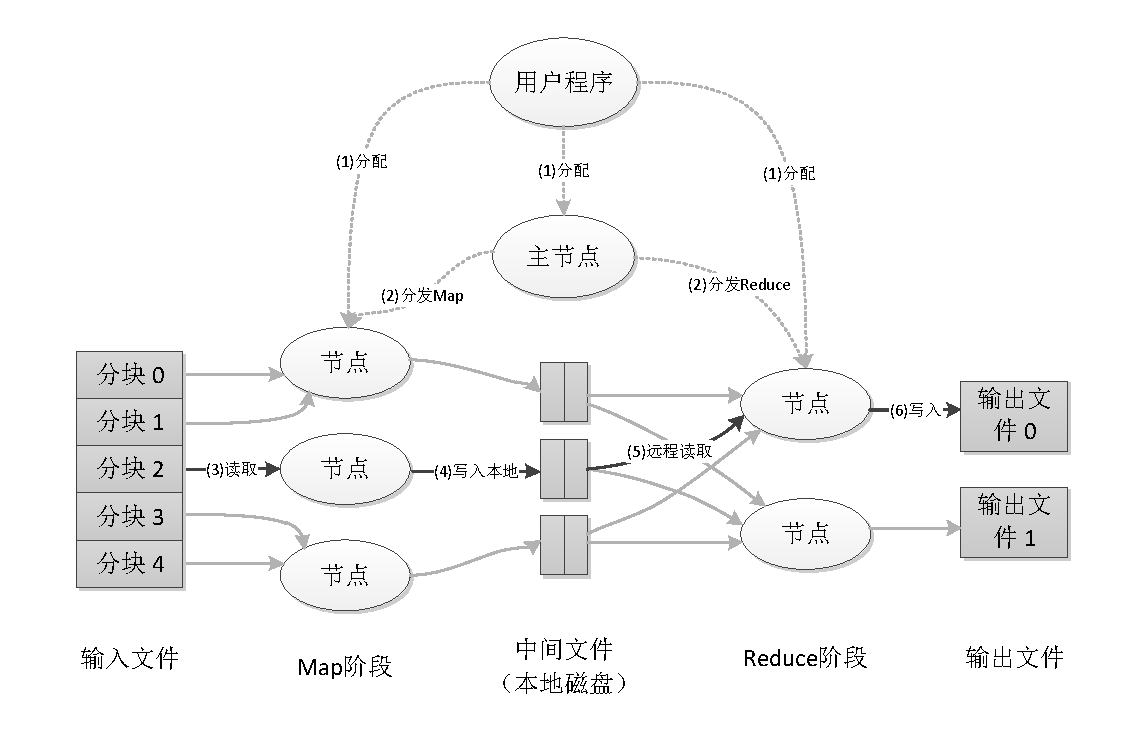
\includegraphics[width=1\textwidth]{MapReduce}
 \caption{MapReduce实现过程}
 \label{fig:MapReduce}
\end{figure}

当用户的程序调用MapReduce的函数的时候,将发生下面的一系列动作(下面的数字和图\ref{fig:MapReduce}中的数字标签相对应):

\begin{enumerate}
\item 在用户程序里的MapReduce库首先分割输入文件成M个片,每个片的大小一般从16到64MB(用户可以通过可选的参数来控制)。然后在机群中开始大量的拷贝程序。

\item 这些程序拷贝中的一个是master,其他的都是由master分配任务的worker。有M个map任务和R个reduce任务将被分配。管理者分配一个map任务或reduce任务给一个空闲的worker。

\item 一个被分配了map任务的worker读取相关输入split的内容。它从输入数据中分析出key/value对,然后把key/value对传递给用户自定义的map函数。由map函数产生的中间key/value对被缓存在内存中。

\item 缓存在内存中的key/value对被周期性的写入到本地磁盘上,通过分割函数把它们写入R个区域。在本地磁盘上的缓存对的位置被传送给master,master负责把这些位置传送给reduce worker。

\item 当一个reduce worker得到master的位置通知的时候,它使用远程过程调用来从map worker的磁盘上读取缓存的数据。当reduce worker读取了所有的中间数据后,它通过排序使具有相同key的内容聚合在一起。因为许多不同的key映射到相同的reduce任务,所以排序是必须的。如果中间数据比内存还大,那么还需要一个外部排序。

\item reduce worker迭代排过序的中间数据,对于遇到的每一个唯一的中间key,它把key和相关的中间value集传递给用户自定义的reduce函数。reduce函数的输出被添加到这个reduce分割的最终的输出文件中。

\item 当所有的map和reduce任务都完成了,管理者唤醒用户程序。在这个时候,在用户程序里的MapReduce调用返回到用户代码。
\end{enumerate}

在成功完成之后,MapReduce执行的输出存放在R个输出文件中(每一个reduce任务产生一个由用户指定名字的文件)。一般,用户不需要合并这R个输出文件成一个文件--他们经常把这些文件当作一个输入传递给其他的MapReduce调用,或者在可以处理多个分割文件的分布式应用中使用他们。

\subsection{MapReduce的优点}
相比于常规分布式程序,MapReduce架构中的分布式程序具有以下几个优点:
\begin{enumerate}

\item MapReduce将并行计算分离成两个独立函数,Map函数和Reduce函数。这种抽象的计算模型将分布式计算从复杂的可模式化的细节管理中剥离出来,使得开发分布式程序变得更加简洁。

\item MapReduce思想来自于函数式编程,架构清晰易懂,入门门槛低,适合于大幅度推广。

\item MapReduce框架轻量,高效,运行过程透明,便与底层的定制和二次开发。

\end{enumerate}


\section{Hadoop}

\subsection[Hadoop简介]{Hadoop简介\cite{book:Hadoop}}
Hadoop是Apache下的一个开源软件,它作为一个开源的软件平台使编写和运行用于处理海量数据的应用程序更加容易。Hadoop框架的核心思想是MapReduce。MapReduce是一个用于进行大数据量计算的编程模型,同时也是一种高效的任务调度模型,它将一个任务分成很多更细粒度的子任务,这些子任务能够在空闺的处理节点之间调度,使处理速度越快的节点处理越多的任务,从而避免处理速度慢的节点延长整个任务的完成时间。

Hadoop是一个能够对大量数据进行分布式处理的软件框架。但是Hadoop是以一种可靠、高效、可伸缩的方式进行处理的。Hadoop是可靠的,因为它假设计算元素和存储会失败,因此它维护多个工作数据副本,确保能够针对失败的节点重新分布处理。Hadoop是高效的,因为它以并行的方式工作,通过并行处理加快处理速度。Hadoop还是可伸缩的,能够处理PB级数据。此外,Hadoop依赖于社区服务器,因此它的成本比较低,任何人都可以使用。

Hadoop由HDFS、MapReduce、HBase、Hive 和ZooKeeper等成员组成。其中,HDFS 和MapReduce 是两个最基础最重要的成员。

\subsection[HDFS的实现]{HDFS的实现\cite{site:hdfs}}
HDFS是分布式计算的存储基石,Hadoop的分布式文件系统和其他分布式文件系统有很多类似的特质。分布式文件系统基本的几个特点:

\begin{enumerate}
\item 对于整个集群有单一的命名空间。
\item 数据一致性。适合一次写入多次读取的模型,客户端在文件没有被成功创建之前无法看到文件存在。
\item 文件会被分割成多个文件块,每个文件块被分配存储到数据节点上,而且根据配置会由复制文件块来保证数据的安全性。
\end{enumerate}

图\ref{fig:HDFS架构}展现了整个HDFS三个重要角色:NameNode、DataNode和Client。

\begin{figure}[h]
 \centering
 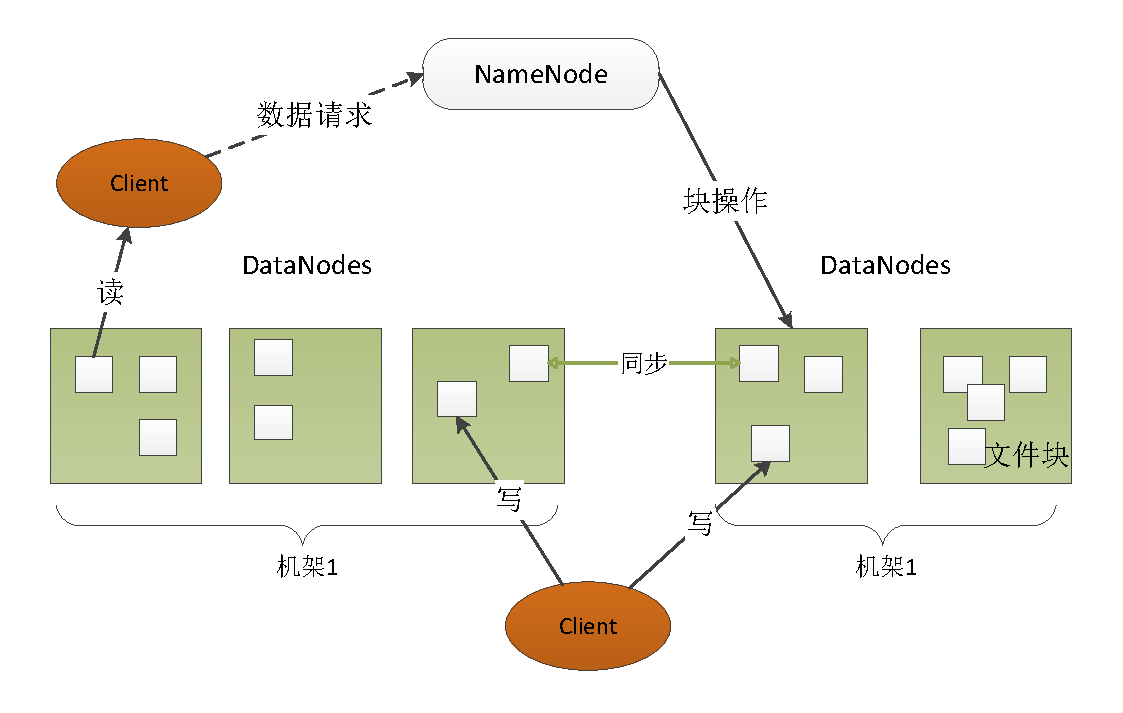
\includegraphics[width=1\textwidth]{HDFS架构}
 \caption{HDFS整体架构图}
 \label{fig:HDFS架构}
\end{figure}

\begin{enumerate}
\item NameNode可以看作是分布式文件系统中的管理者,主要负责管理文件系统的命名空间、集群配置信息和存储块的复制等。NameNode会将文件系统的Meta-data存储在内存中,这些信息主要包括了文件信息、每一个文件对应的文件块的信息和每一个文件块在DataNode的信息等。
\item DataNode是文件存储的基本单元,它将Block存储在本地文件系统中,保存了Block的Meta-data,同时周期性地将所有存在的Block信息发送给NameNode。
\item Client就是需要获取分布式文件系统文件的应用程序。这里通过三个操作来说明他们之间的交互关系。
\end{enumerate}

文件写入:

\begin{enumerate}
\item Client向NameNode发起文件写入的请求。
\item NameNode根据文件大小和文件块配置情况,返回给Client它所管理部分DataNode的信息。
\item Client将文件划分为多个Block,根据DataNode的地址信息,按顺序写入到每一个DataNode块中。
\end{enumerate}

文件读取:

\begin{enumerate}
\item Client向NameNode发起文件读取的请求。
\item NameNode返回文件存储的DataNode的信息。
\item Client读取文件信息。
\end{enumerate}

文件Block复制:

\begin{enumerate}
\item NameNode发现部分文件的Block不符合最小复制数或者部分DataNode失效。
\item 通知DataNode相互复制Block。
\item DataNode开始直接相互复制。
\end{enumerate}

因此,HDFS具有以下的几个设计特点:

\begin{enumerate}
\item Block的放置:默认不配置。一个Block会有三份备份,一份放在NameNode指定的DataNode,另一份放在与指定DataNode非同一Rack上的DataNode,最后一份放在与指定DataNode同一Rack上的DataNode上。备份无非就是为了数据安全,考虑同一Rack的失败情况以及不同Rack之间数据拷贝性能问题就采用这种配置方式。
\item 心跳检测DataNode的健康状况,如果发现问题就采取数据备份的方式来保证数据的安全性。
\item 数据复制(场景为DataNode失败、需要平衡DataNode的存储利用率和需要平衡DataNode数据交互压力等情况):这里先说一下,使用HDFS的balancer命令,可以配置一个Threshold来平衡每一个DataNode磁盘利用率。例如设置了Threshold为10%,那么执行balancer命令的时候,首先统计所有DataNode的磁盘利用率的均值,然后判断如果某一个DataNode的磁盘利用率超过这个均值Threshold以上,那么将会把这个DataNode的block转移到磁盘利用率低的DataNode,这对于新节点的加入来说十分有用。
\item 数据交验:采用CRC32作数据交验。在文件Block写入的时候除了写入数据还会写入交验信息,在读取的时候需要交验后再读入。
\item NameNode是单点:如果失败的话,任务处理信息将会纪录在本地文件系统和远端的文件系统中。
\item 数据管道性的写入:当客户端要写入文件到DataNode上,首先客户端读取一个Block然后写到第一个DataNode上,然后由第一个DataNode传递到备份的DataNode上,一直到所有需要写入这个Block的NataNode都成功写入,客户端才会继续开始写下一个Block。
\item 安全模式:在分布式文件系统启动的时候,开始的时候会有安全模式,当分布式文件系统处于安全模式的情况下,文件系统中的内容不允许修改也不允许删除,直到安全模式结束。安全模式主要是为了系统启动的时候检查各个DataNode上数据块的有效性,同时根据策略必要的复制或者删除部分数据块。运行期通过命令也可以进入安全模式。在实践过程中,系统启动的时候去修改和删除文件也会有安全模式不允许修改的出错提示,只需要等待一会儿即可。
\end{enumerate}

HDFS是MapReduce的读写的底层实现,对MapReduce进化起着至关重要的作用。

\subsection[Hadoop的运行过程]{Hadoop的运行过程\cite{book:Hadoop}}
在Hadoop的系统中,会有一台Master,主要负责NameNode的工作以及JobTracker的工作。JobTracker的主要职责就是启动、跟踪和调度各个Slave的任务执行。还会有多台Slave,每一台Slave通常具有DataNode的功能并负责TaskTracker的工作。TaskTracker根据应用要求来结合本地数据执行Map任务以及Reduce任务。

具体如图\ref{fig:Hadoop运行流程}所示,过程如下:

\begin{enumerate}
\item 在分布式环境中客户端创建任务并提交。

\item InputFormat做Map前的预处理,主要负责以下工作:

1)验证输入的格式是否符合JobConfig的输入定义,这个在实现Map和构建Conf的时候就会知道,不定义可以是Writable的任意子类。

2)将input的文件切分为逻辑上的输入InputSplit,其实这就是在上面提到的在分布式文件系统中blocksize是有大小限制的,因此大文件会被划分为多个block。

3)通过RecordReader来再次处理inputsplit为一组records,输出给Map。inputsplit只是逻辑切分的第一步,但是如何根据文件中的信息来切分还需要RecordReader来实现,例如最简单的默认方式就是回车换行的切分。

\item RecordReader处理后的结果作为Map的输入,Map执行定义的Map逻辑,输出处理后的key和value对应到临时中间文件。

\item Combiner可选择配置,主要作用是在每一个Map执行完分析以后,在本地优先作Reduce的工作,减少在Reduce过程中的数据传输量。

\item Partitioner可选择配置,主要作用是在多个Reduce的情况下,指定Map的结果由某一个Reduce处理,每一个Reduce都会有单独的输出文件。(后面的代码实例中有介绍使用场景)

\item Reduce执行具体的业务逻辑,并且将处理结果输出给OutputFormat。

\item OutputFormat的职责是,验证输出目录是否已经存在,同时验证输出结果类型是否如Config中配置,最后输出Reduce汇总后的结果。
\end{enumerate}

\begin{figure}
 \centering
 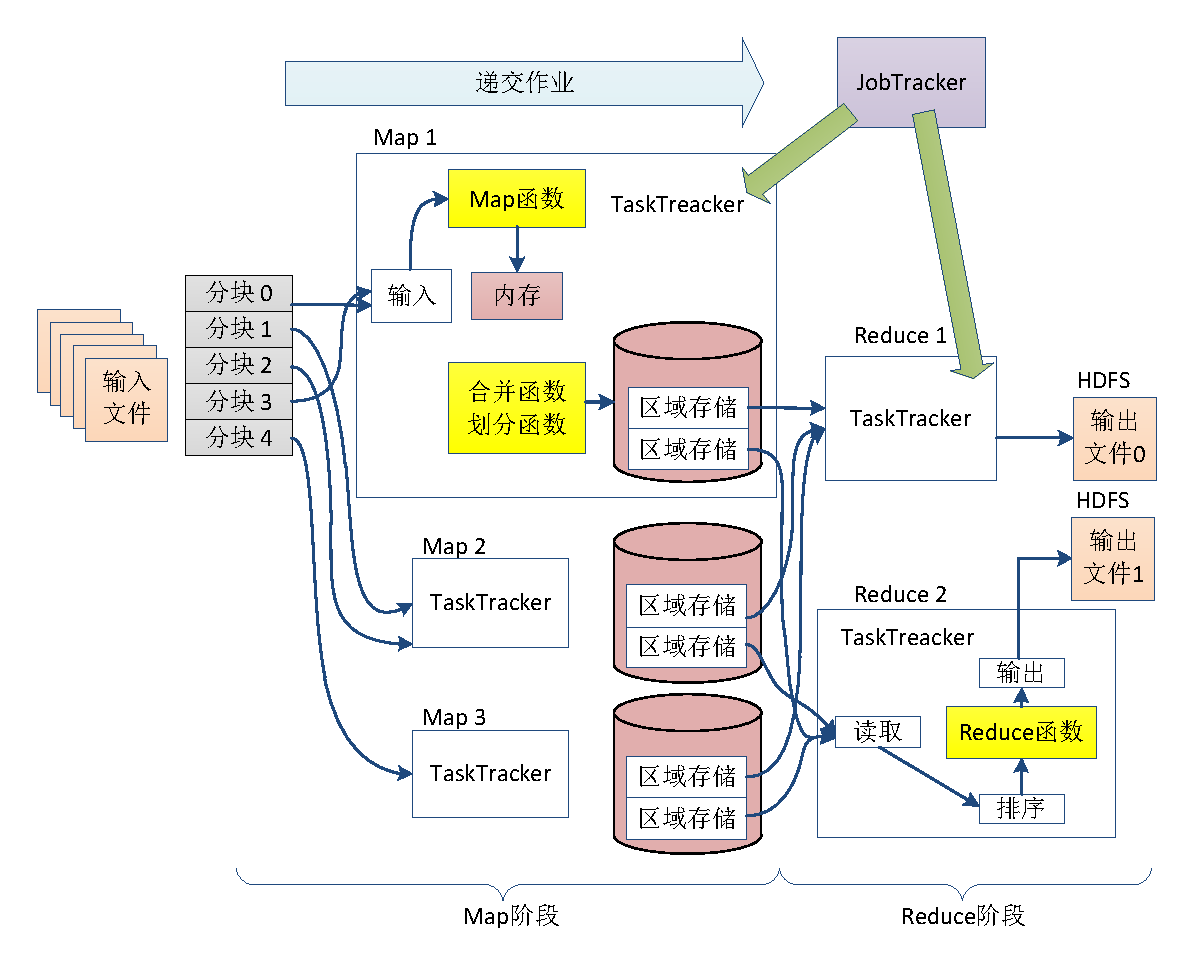
\includegraphics[width=1\textwidth]{Hadoop运行流程}
 \caption{Hadoop运行流程}
 \label{fig:Hadoop运行流程}
\end{figure}

\subsection{Hadoop的组成}
Hadoop整体功能由五个子进程实现,他们分别为NameNode、SecondaryNameNode、Jobtracker、DataNode和TaskTracker,其具体功能如下:

NameNode,NameNode是分布式文件系统的管理者,主要负责文件系统的命名空间,集群的配置信息和数据块的复制信息等,并将文件系统的元数据存储在内存中。

SecondaryNameNode,SecondaryNameNode有两个作用,一是镜像备份,二是日志与镜像的定期合并。它会周期性的将EditLog中记录的对HDFS的操作合并到一个checkpoint中,然后清空EditLog。如果没有SecondaryNameNode的这个周期性的合并过程,那么当每次重启NameNode的时候,就会花费很长的时间。而这样周期性的合并就能减少重启的时间。同时也能保证HDFS系统的完整性。

JobTracker,负责任务的接受初始化,调度以及对TaskTrackee的监控。JobTracker作为一个单独的JVM运行,对整个MapReduce程序的运行起着至关重要的作用。

DataNode,负责为响应来自HDFS客户机的读写请求。它们还响应创建、删除和复制来自NameNode的块的命令。并与NameNode通过心跳包来维持联系。DataNode,负责为响应来自是文件实际存储的位置,它将块(Block)的元数据信息存储在本地文件系统中,周期性地将所有的Block信息发给NameNode。

TaskTrackee,运行作业划分后的任务。

其中NameNode、SecondaryNameNode和Jobtracker运行在Master节点上,DataNode和TaskTracker运行在Slave节点上。

本文中,因为实验环境限制,Hadoop运行模式为伪分布式,即五个子进程均处于同一宿主机上。如图\ref{fig:五个子进程}

\begin{figure}[h]
 \centering
 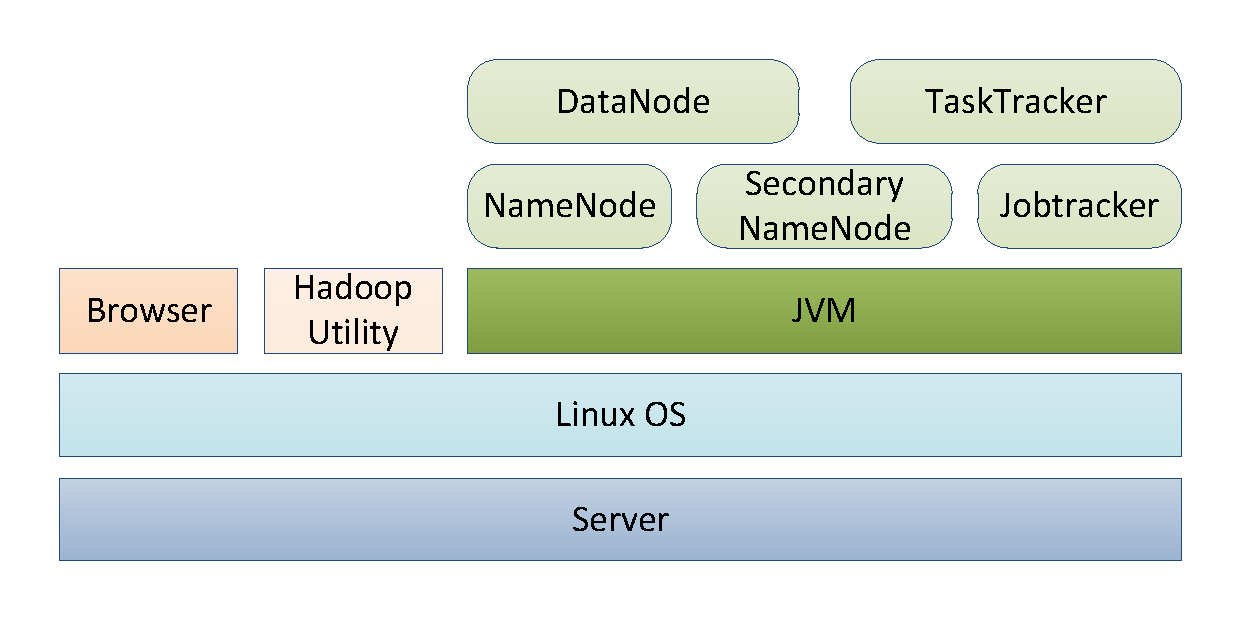
\includegraphics[width=0.9\textwidth]{五个子进程}
 \caption{五个子进程与操作系统的结构}
 \label{fig:五个子进程}
\end{figure}
%Hadoop基于SSH协议管理集群,节点间通过HDFS传输文件,程序运行时,Hadoop中的JobTracker守护进程负责调度节点,将Map和Reduce按照一定的规则分发到节点上的TaskTracker进程中,TaskTracker进程根据编写好的Map函数和Reduce函数从HDFS上获取数据并对其做进一步的处理。

%Mapper将HDFS中的文件按照事先编写好的Map函数进行处理,并将处理结果以Key/Value对的形式输出,之后,Hadoop会把Map结果根据键值合并,并将合并结果分发到集群用Reduce函数处理。这个过程中的整体通信会带来很大的网络I/O开销,尤其是在Map的开始和结束的时候,会带来一场大的“网络风暴”。同时,Hadoop会在运行时产生临时文件,从而带来很大的内存和磁盘开销。

%因此,运行Hadoop的机器应具有网络吞吐量好,可用内存大,磁盘读写速度快三个特点。

\subsection{Hadoop的特点}
Hadoop是面向大型集群实现MapReduce方法而设计的编程框架,其实现具有以下几个特点。

\begin{enumerate}
\item 可扩展:不论是存储的可扩展还是计算的可扩展都是Hadoop的设计根本。Hadoop中许多组件都是可插拔的,如调度器

\item 经济:框架可以运行在任何普通的PC上,使用者只需使用普通的PC机即可搭建性能强大的集群。

\item 可靠:分布式文件系统的备份恢复机制以及MapReduce的任务监控保证了分布式处理的可靠性。

\item 高效:分布式文件系统的高效数据交互实现以及MapReduce结合Local Data处理的模式,为高效处理海量的信息作了基础准备。

\item 使用方便:Hadoop使用Java语言实现,利用ssh协议与各节点之间通信,底层依赖小,可移植性强,适应于各种环境。
\end{enumerate}

\subsection{MapReduce在Hadoop中的三种实现方式及特点}

1. 原生Java
Hadoop是用Java编写的,所有Hadoop文件系统间的相互作用都是由Java API调解的。 举个例子,文件系统的shell就是一个Java应用,它使用Java文件系统类来提供文件系统操作。

同时,Hadoop提供了一套完整的Java类,用以实现MapReduce、HDFS操作及Hadoop配置。实际开发过程中,开发者可以直接引用这些类,达到快速开发的目的。

2. Streaming
Streaming框架允许任何程序语言实现的程序在Hadoop MapReduce中使用,方便已有程序向Hadoop平台移植。其原理是用Java实现一个包装用户程序的MapReduce程序,该程序负责调用MapReduce Java接口获取key/value对输入,创建一个新的进程启动包装的用户程序,将数据通过管道传递给包装的用户程序处理,然后调用MapReduce Java接口将用户程序的输出切分成key/value对输出。

Streaming天生适合用于文本处理(到0.21.0版本时,Streaming也可以处理二进制流),在文本模式下使用时,它有一个数据的行视图。map的输入数据通过标准输入流传递给map函数,并且是一行一行地传输,最后将结果行写到标准输出。map输出的键/值对是以一个制表符分隔的行,它以这样的形式写到标准输出。reduce 函数的输入格式相同——通过制表符来分隔的键/值对——并通过标准输入流进行传输。reduce函数从标准输入流中读取输入行,该输入已由Hadoop框架根据键排过序,最后将结果写入标准输出。

Streaming和Java MapReduce API在设计时有一些差异:Java API控制的map函数一次只能处理一条记录。针对输入数据中的每一条记录,该框架均需调用Mapper的map()方法来处理,然而在Streaming中,map程序可以自己决定如何处理输入数据,例如,它可以轻松读取并同时处理若干行,因为它受读操作的控制。用户的Java map实现的是“推”记录方式,但它依旧可以同时处理多行,具体做法是通过mapper中实例变量将之前读取的多行汇聚在一起。在这种情况下,需要实现close()方法,以便知道何时读到最后一条记录,进而完成对最后一组记录行的处理。

如下图\ref{fig:Streaming}所示,其中Streaming Java Mapper通过管道将key/value输入传递给用户mapper程序的标准输入,并获取用户mapper程序的标准输出;Streaming Java Reducer调用Java接口通过InputFormat从HDFS获取输入数据,从管道将key/value传递给用户 reducer程序的标准输入,获取用户reducer程序的标准输出并调用Java接口通过OutputFormat输出数据;用户mapper和reducer程序负责处理数据,都从标准输入读取数据,向标准输出写入数据。


\begin{figure}[h]
 \centering
 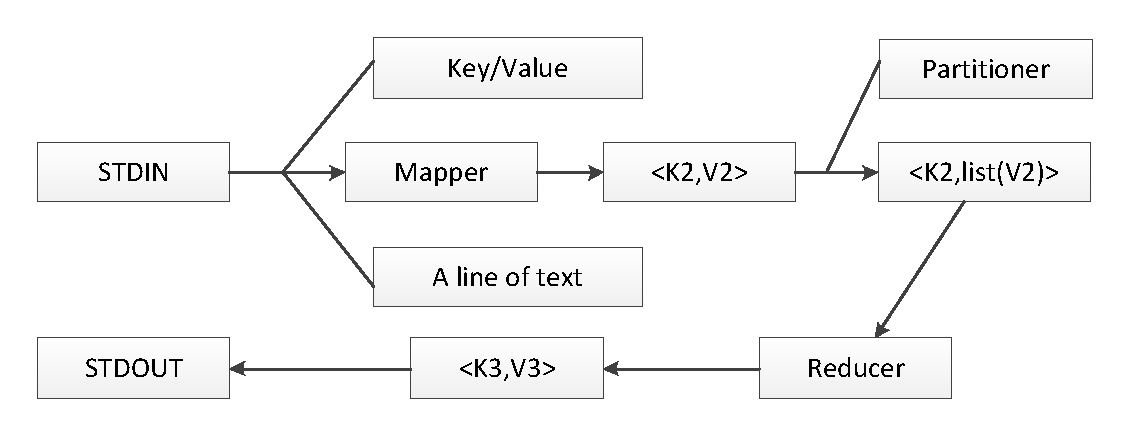
\includegraphics[width=1\textwidth]{Streaming}
 \caption{Streaming运行流程图}
 \label{fig:Streaming}
\end{figure}


Streaming有如下一些优点: 

\begin{enumerate}
\item 开发效率高,很多现有程序(包括脚本)能够方便的移植到hadoop平台上去运行 

\item 某些程序运行效率高,对于某些cpu密集型程序,如果map-reduce程序用C++编写,效率有可能提高 
\end{enumerate}

Streaming存在如下一些不足:

\begin{enumerate}
\item Streaming中的mapper和reducer默认只能向标准输出写数据,不能方便地处理多路输出。 

\item 用Java编写的MapReduce程序直接处理框架从输入数据中得到的key/value对,在Streaming中Java程序不直接处理key/value对,而是通过管道写到mapper程序的标准输入,mapper程序再从key/tvalue中解析出key/value对,这个过程多了两次数据拷贝和解析(分割),带来一定的开销。对于reducer也是一样的。
\end{enumerate}

3. Pipes

Hadoop的Pipes是Hadoop MapReduce的C++接口代称。不同于使用标准输入和输出来实现map代码和reduce代码之间的Streaming,Pipes使用套接字作为tasktracker与C++版本map函数或reduce函数的进程之间的通道。

应用程序对Hadoop C++库链接提供了一个与tasktracker 子进程进行通信的简单封装。通过扩展HadoopPipes命名空间中定义的mapper和reducer两个类,定义了map()和reduce()方法,同时MapReduce提供各种情况下map()和reduce()方法的实现。这些方法采用了上下文对象(MapContext类型或ReduceContext类型),进而提供了读取输入数据和写入输出数据,以及通过JobConf类来访问作业配置信息的功能。

与Java接口不同,C++接口中的键和值按字节缓冲,用标准模板库(Standard Template Library,STL)中的字符串表示。这样做简化了接口,但把更重的负担留给了应用程序开发人员,因为开发人员必须来回封送(marshall)字符串与特定应用领域内使用的具体类型。

因Pipes通过trasktracker子进程进行通信,但由于Hadoop提供的C++接口功能过于简单,开发负担大,故本文中仅对原生Java和Streaming的实现做性能对比。

\subsection[Hadoop计数器及其含义]{Hadoop计数器及其含义\cite{site:hadoop-counter}}
Hadoop里有一个很常用的工具叫计数器(Counter), 主要用来记录Hadoop job的运行状态。通过计数器,用户可以观察MapReduce job运行期间的各个细节数据,大多数优化都是基于计数器的数值表现。本文中后期的性能分析主要依靠Hadoop计数器提供的数据完成。

Hadoop job提供的默认计数器分为五个组分别是Job Counters、File Input Format Counters、File Output Format Counters、FileSystem Counters和Map-Reduce Framework其包含的数据和含义如下:

\begin{enumerate}

\item Job Counters 

这个计数器描述与job调度相关的统计 

Data-local map tasks:Job在被调度时,如果启动了一个data-local(源文件的幅本在执行map task的taskTracker本地) 

FALLOW\_SLOTS\_MILLIS\_MAPS:当前job为某些map task的执行保留了slot,总共保留的时间是多少 

FALLOW\_SLOTS\_MILLIS\_REDUCES:与上面类似 

SLOTS\_MILLIS\_MAPS:所有map task占用slot的总时间,包含执行时间和创建/销毁子JVM的时间 

SLOTS\_MILLIS\_REDUCES:与上面类似 

Launched map tasks:此job启动了多少个map task 

Launched reduce tasks:此job启动了多少个reduce task 


\item File Inut Format Counters

这个计数器表示map task读取文件内容(总输入数据)的统计

BYTES\_READ:Map task的所有输入数据(字节),等于各个map task的map方法传入的所有value值字节之和。 

\item File Output Format Counters

这个计数器表示map task写入文件内容(总输入数据)的统计

BYTES\_READ:Map task的所有输出数据(字节),等于各个map task的map方法传出的所有value值字节之和。 

\item FileSystem Counters

MapReduce job执行所依赖的数据来自于不同的文件系统,这个计数器表示job与文件系统交互的读写统计 

FILE\_BYTES\_READ:job读取本地文件系统的文件字节数。假定当前map的输入数据都来自于HDFS,那么在map阶段,这个数据应该是0。但reduce在执行前,它的输入数据是经过shuffle的merge后存储在reduce端本地磁盘中,所以这个数据就是所有reduce的总输入字节数。 

FILE\_BYTES\_WRITTEN:map的中间结果都会spill到本地磁盘中,在map执行完后,形成最终的spill文件。所以map端这里的数据就表示map task往本地磁盘中总共写了多少字节。与map端相对应的是,reduce端在shuffle时,会不断地拉取map端的中间结果,然后做merge并不断spill到自己的本地磁盘中。最终形成一个单独文件,这个文件就是reduce的输入文件。 

HDFS\_BYTES\_READ:整个job执行过程中,只有map端运行时,才从HDFS读取数据,这些数据不限于源文件内容,还包括所有map的split元数据。所以这个值应该比FileInputFormatCounters.BYTES\_READ 要略大些。 

HDFS\_BYTES\_WRITTEN:Reduce的最终结果都会写入HDFS,就是一个job执行结果的总量。 


\item Map-Reduce Framework

这个计数器包含了相当多地job执行细节数据。这里需要有个概念认识是:一般情况下,record就表示一行数据,而相对地byte表示这行数据的大小是多少,这里的计数器表示经过reduce merge后像这样的输入形式{“aaa”, [5, 8, 2, …]}。 

Combine input records:Combiner是为了减少尽量减少需要拉取和移动的数据,所以combine输入条数与map的输出条数是一致的。 

Combine output records:经过Combiner后,相同key的数据经过压缩,在map端自己解决了很多重复数据,表示最终在map端中间文件中的所有条目数 

Failed Shuffles:copy线程在抓取map端中间数据时,如果因为网络连接异常或是IO异常,所引起的shuffle错误次数 

GC time elapsed(ms):通过JMX获取到执行map与reduce的子JVM总共的GC时间消耗 

Map input records:所有map task从HDFS读取的文件总行数 

Map output records:map task的直接输出record是多少,就是在map方法中调用context.write的次数,也就是未经过Combine时的原生输出条数 

Map output bytes:Map的输出结果key/value都会被序列化到内存缓冲区中,所以这里的bytes指序列化后的最终字节之和 

Merged Map outputs:记录着shuffle过程中总共经历了多少次merge动作 

Reduce input groups:Reduce总共读取了多少个这样的计数器 

Reduce input records:如果有Combiner的话,那么这里的数值就等于map端Combiner运算后的最后条数,如果没有,那么就应该等于map的输出条数 

Reduce output records:所有reduce执行后输出的总条目数 

Reduce shuffle bytes:Reduce端的copy线程总共从map端抓取了多少的中间数据,表示各个map task最终的中间文件总和 

Shuffled Maps:每个reduce几乎都得从所有map端拉取数据,每个copy线程拉取成功一个map的数据,那么增1,所以它的总数基本等于 reduce number * map number 

Spilled Records:spill过程在map和reduce端都会发生,这里统计在总共从内存往磁盘中spill了多少条数据 

SPLIT\_RAW\_BYTES 
与map task 的split相关的数据都会保存于HDFS中,而在保存时元数据也相应地存储着数据是以怎样的压缩方式放入的,它的具体类型是什么,这些额外的数据是MapReduce框架加入的,与job无关,这里记录的大小就是表示额外信息的字节大小 

\end{enumerate}
	
	
\section[Web访问日志简介]{Web访问日志简介\cite{site:weblog}}
\subsection{什么是Web访问日志}
Web访问日志是Web服务器的运行记录文档,当用户访问一个网站时,服务器上的Web服务会接受该用户的请求,并将用户的请求信息记录并保存下来。目前常见的Web访问日志格式主要由两类,一类是Apache的NCSA日志格式,另一类是IIS的W3C日志格式。NCSA格式又分为NCSA普通日志格式(CLF)和NCSA扩展日志格式(ECLF)两类,目前最常用的是NCSA扩展日志格式(ECLF)及基于自定义类型的Apache日志格式;而W3C扩展日志格式(ExLF)具备了更为丰富的输出信息,但目前的应用并不广泛。目前,大多数网站使用NCSA日志格式来存储日志。

Nginx是一款基于Epoll模型的web服务程序\cite{site:nginx},近年来发展迅猛,截止2012年5月,Nginx已经占据Web软件10.32\%的份额\cite{site:netcraft_nginx},Nginx的默认日志为Apache的NCSA扩展日志格式(ECLF),本实验中所用的日志为Nginx默认生成的日志。

\subsection{NCSA扩展日志格式的组成}
这是一个最常见的基于NCSA扩展日志格式(ECLF)的Nginx日志样例:

\begin{verbatim}
222.25.151.30 - - [28/May/2012:19:12:03 +0800] "GET /bbs/uc_server/ava
tar.php?uid=46369&size=small HTTP/1.1" 301 0 "http://rs.xidian.edu.cn/
bbs/index.php" "Mozilla/4.0 (compatible; MSIE 8.0; Windows NT 5.1; Tri
dent/4.0; GTB7.2; .NET CLR 1.1.4322; .NET CLR 2.0.50727; CIBA; TheWorl
d)" -
\end{verbatim}

可以很清楚的看到,这个日志主要由以下几个部分组成:

\begin{enumerate}
\item 访问主机(remotehost)

显示主机的IP地址或者已解析的域名。

\item 标识符(Ident)

由identd或直接由浏览器返回浏览者的EMAIL或其他唯一标示,因为涉及用户邮箱等隐私信息,目前几乎所有的浏览器就取消了这项功能。

\item 授权用户(authuser)

用于记录浏览者进行身份验证时提供的名字,如果需要身份验证或者访问密码保护的信息则这项不为空,但目前大多数网站的日志这项也都是为空的。

\item 日期时间(date)

一般的格式形如[22/Feb/2010:09:51:46 +0800],即[日期/月份/年份:小时:分钟:秒钟 时区],占用的的字符位数也基本固定。

\item 请求(request)

即在网站上通过何种方式获取了哪些信息,也是日志中较为重要的一项,主要包括以下三个部分:


\item 请求类型(METHOD)

常见的请求类型主要包括GET/POST/HEAD这三种;


\item 请求资源(RESOURCE)


显示的是相应资源的URL,可以是某个网页的地址,也可以是网页上调用的图片、动画、CSS等资源,是Web访问日志挖掘中的一个重点;


\item 协议版本号(PROTOCOL)


显示协议及版本信息,通常是HTTP/1.1或HTTP/1.0。

\item 状态码(status)

用于表示服务器的响应状态,通常1xx的状态码表示继续消息;2xx表示请求成功;3xx表示请求的重定向;4xx表示客户端错误;5xx表示服务器错误。

\item 传输字节数(bytes)

即该次请求中一共传输的字节数。

\item 来源页面(referrer)

用于表示浏览者在访问该页面之前所浏览的页面,只有从上一页面链接过来的请求才会有该项输出,如果是新开的页面则该项为空。上例中来源页面是google,即用户从google搜索的结果中点击进入。

\item 用户代理(agent)

用于显示用户的详细信息,包括IP、OS、Bowser等。

\end{enumerate}

\subsection{Web访问日志的作用及价值}
Web访问日志记录了用户访问一个网站的所有过程,是个非常好的数据挖掘原料。通过对Web访问日志的分析,网站服务提供商可以获得某一指定用户的点击流(Clickstream),网站的流量及访问时段,网站的内部漏洞及可能的注入点。

有效的利用Web访问日志可以高效精准的分析出用户喜好,帮助网站运营商提升网站质量。

\section{本章小结}
本章主要介绍本文的研究背景,详述了MapReduce、Hadoop的起源、发展及其运行机制,并详述了Hadoop Counter和Web访问日志的内容及其格式。为进一步的开发和研究做了铺垫。
    \chapter{基于Hadoop的MapReduce程序设计}
\label{chap:3}

\section{Web访问日志分析程序设计}
\subsection{程序应用场景}
随着互联网的高速发展,各种Web2.0网站、电子商务网站创造了前所未有的访问记录,各种大型网络游戏不断刷新着在线用户数峰值,与此同时这些大型系统都记录下了海量的运行日志。挖掘出日志中蕴藏的信息来改进用户体验提升服务质量是非常有价值的。本程序利用MapReduce框架,利用分布式集群处理访问日志计算PV,可以解决传统生产环境中单机处理Web访问日志速度过慢的问题。

\subsection{程序实现过程}
本程序基于Hadoop 1.0.1,利用MapReduce思想进行程序开发。MapReduce思想十分简单,首先将所有的数据分发到各个集群上,并在集群执行Map函数,之后将Map结果合并并交给reduce做进一步的计算,详见本文第\ref{chap:2}章。

根据MapReduce思想,根据实际需求,本程序运行流程图如图\ref{fig:程序流程图}所示:

\begin{figure}[h]
 \centering
 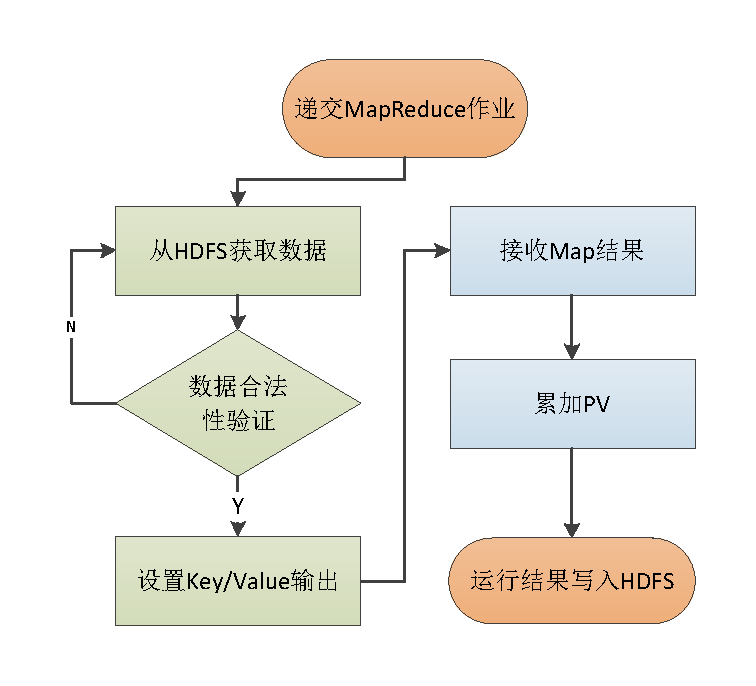
\includegraphics[width=0.7\textwidth]{程序流程图}
 \caption{程序流程图}
 \label{fig:程序流程图}
\end{figure}

Map函数的功能为:从HDFS上获取日志文件,文件每一行作为一个输入,Mapper在读取行之后,验证其访问的有效性,之后设置“pv”作为Mapper的key,1作为值,将Map结果输出。Reduce函数的功能为:从Map端接收合并好的Key/Value对,将key所对应的Value的值相加,得到PV值,将新的Key/Value对输出。



\subsection{程序运行环境}
Hadoop依赖SSH和JDK,具有很高的通用性,但一般情况下,为了整体集群的效率,操作系统一般选用Linux,使用Sun JDK,本程序的开发运行环境具体如下:

实验机器配置:

CPU:Pentium(R) Dual-Core  CPU E5800 @ 3.20GHz

内存:2G DDR2 800

硬盘:Seagate 320G 7200RPM

操作系统:CentOS\_6.2\_x64
  
CentOS是RedHat的开源版本,具有了RedHat的一切特性并有着稳定的社区支持,以其高效和稳定著称,是理想的Hadoop宿主操作系统。6.2是其最新稳定版。本文中所使用的CentOS为netinstall版,这种方式安装出来的CentOS体积最小,软件包最新,服务数量最少,运行速度最快,且不损失任何系统稳定性。

JDK:Sun JDK 1.6.0\_31

Java Development Kit (JDK) 是Sun公司针对Java开发人员发布的免费软件开发工具包(SDK,Software development kit)。自从Java推出以来,Sun JDK已经成为使用最广泛的Java SDK。1.6.0\_31是其最新稳定版。

Hadoop 1.0.1

Hadoop是Apache社区下的开源软件,1.0.1是其最新稳定版。

编程语言:Java、Python 2.6

编程语言的差异会对程序的运行效率产生至关重要的影响,本实验选用Java、Python两种最常见的解释性编程语言,便于后期性能对比。


\section{程序开发与实现}
\subsection{原生Java的实现}
Hadoop使用Java语言实现,其自身提供了一套完整的Java类库,使用起来十分方便。

首先,创建一个Java文件,在文件头部定义package名称,引入相关类库之后就可以开始编写Mapreduce程序了,程序中需要在Java包内定一个一个Public类pv,运行时,将类名作为参数传入Hadoop。pv类里定义Map和Reduce类和一个main函数:TokenizerMapper继承Mapper类,IntSumReducer继承Reducer类,main函数里指定运行的Map和Reduce类名、和数据类型,其各部分具体功能如下:

TokenizerMapper定义两个private变量,用于存储Key/Value的值。之后定义一个map函数,判断读入的数据的合法性,若合法,则给value赋值1,反之赋值0。

IntSumReducer定义一个变量,用于存储最终pv的值。之后定一个一个函数reducer,将Map传入的结果累加。最后输出Key和pv值。

main函数中实例化Hadoop的配置类、和Job类,并给job类的各项属性赋值。

编写完毕之后,应对程序进行调试,Hadoop为Eclipse提供了完整的调试插件,但由于其配置复杂且超出了本文讨论范围,在此不详细给出。

其在Hadoop中的运行流程如下:

至此,Web日志处理的原生Java程序就实现了。

\subsection{基于Streaming的Python实现}
Hadoop在支持原生Java的同时也对外提供了Streaming方法,该方法把HDFS中的文件转化成文件流,传入外部程序处理,使得Hadoop具有处理非Java编写的程序的能力。本文选用了和Java及其类似的解释性编程语言Python,便于后期的性能测试对比。

在Hadoop的Streaming中,所编程序在开发过程中无需引用任何Hadoop类库,Hadoop会将文件转换成文件流输入,程序处理之后,再将Key/Value对以std方式输出,Hadoop会自动捕获输出并进行下一步处理。实现是,Mapper和Reducer需要单独书写。

新建文件Mapper.py,文件首部向系统声明文件执行类型为python,又因程序使用std I/O并分割字符串,所以在头部引用sys和itemgetter。之后使用for循环语句从sys.stdin读取数据,并判断其合法性,若合法,则给value赋值1,反之赋值0,最后使用print输出Key/Value对,并以一个缩进符号分割开来。

新建文件Reducer.py,文件首部和引用于Mapper.py相同,定义存储pv值的变量sum,使用for循环从sys.stdin读取Mapper中生成的文件流,使用itemgetter分割Key/Value对到对应的变量,将pv值累加。最后使用print输出Key和pv值。

由于Streaming使用std I/O,使得其调试非常简单,用户可以直接在本机使用cat命令通过Unix管道即可进行简单的的调试。运行命令cat 10.log | ./mapper.py即可查看Map的结果。运行cat 10.log | ./mapper.py | ./reducer.py即可查看MapReducer结果。

运行时向hadoop指定map文件和reduce文件,并使用file命令将map/reduce程序分发到各节点即可。


其在Hadoop中的运行流程如下:

至此,Web日志处理的Python程序就实现了。

\section{实现效果及性能测试}
\subsection{测试数据及方法}
为了验证本程序的正确性和运行效率,笔者使用了9组数据,测试数据为基数为10到100,000,000,增量为十倍,共8组清洗过的有效合法日志,日志取自实际生产环境服务器,具有一定的参考价值。所有测试数据均存放在采用Hadoop默认配置的HDFS上。

测试环境为伪分布式的单机Hadoop节点,Java和Python程序的运行均使用Hadoop默认参数执行,测试过程中,使用sar对系统资源进行监测,测试结束后,收集运行日志进行更进一步的分析。


\subsection{基于原生Java的实现及性能测试}
本实验中Java程序均使用Sun\_JDK\_1.6.0\_31编译并打包,Java程序上传到服务器上之后,执行命令

\begin{verbatim}
hadoop jar pv.jar test.pv input/100.log output/java/100
\end{verbatim}

其中pv.jar为打包后的程序,test.pv为程序中所对应的包及类,input/100.log为HDFS上的日志文件, output/java/100为输出目录。

命令执行后,终端会实时跟踪程序运行情况,用户也可以通过网页终端查看当前程序的运行状况。程序执行完毕之后,Hadoop会将程序运行信息输出至终端,程序运行结果保存在指定的HDFS目录下用户可以运行一下命令查看运行结果。

\begin{verbatim}
hadoop dfs -cat output/java/100/part-r-00000
\end{verbatim}

在本实验中,所用测试数据是提前使用工具处理好的数据,目的在于验证程序的准确性并分析对比其运行时间。具体运行结果和运行时间如下表:

\subsection{基于Streaming的Python实现及其性能测试}

本实验中的Python程序均使用CentOS自带的Python 2.6.6解析,Python程序上传到服务器上之后,执行命令

\begin{verbatim}
hadoop jar $HADOOP_HOME/contrib/streaming/hadoop-streaming-1.0.1.jar \
-file mapper.py -mapper mapper.py \
-file reducer.py -reducer reducer.py \
-input input/100.log -output output/python/100
\end{verbatim}

其中\$HADOOP\_HOME/contrib/streaming/hadoop\-streaming\-1.0.1.jar为Hadoop内置的Streaming类,\-file命令将程序分发到各节点,\-mapper和\-reducer命令分别制定mapper.py和reducer.py为Mapper和Reducer,input/100.log为HDFS上的日志文件, output/python/100为输出目录。

命令执行后,同原生Java一样,终端会实时跟踪程序运行情况,用户也可以通过网页终端查看当前程序的运行状况。程序执行完毕之后,Hadoop会将程序运行信息输出至终端,程序运行结果保存在指定的HDFS目录下用户可以运行一下命令查看运行结果。

\begin{verbatim}
hadoop dfs -cat output/python/100/part-r-00000
\end{verbatim}

同上一小节,在本实验中,所用测试数据是提前使用工具处理好的数据,目的在于验证程序的准确性并分析对比其运行时间。具体运行结果和运行时间如下表:


\section{本章小结}
本章以Web访问日志程序开发为例,分别介绍了在Hadoop下的两种程序开发模式:原生Java和Streaming,并对其性能做了测试,下一章会根据本章第三节的测试结果做以分析和说明。
    \chapter{基于Hadoop的MapReduce实现的性能分析}
\label{chap:4}

\section{Hadoop调度对性能的影响}
Hadoop程序运行时,会有进程监控节点资源,并将系统中的空闲资源按一定的策略分配给作业,这个进程的核心就是调度器。Hadoop默认的调度器是JobQueueTaskScheduler,使用规则为FIFO (First In First Out,即先入先出)原则,即按照作业的优先级高低,再按照到达时间的先后选择被执行的作业。

其具体工作流程如下图\ref{fig:调度器}:
\begin{figure}[h]
 \centering
 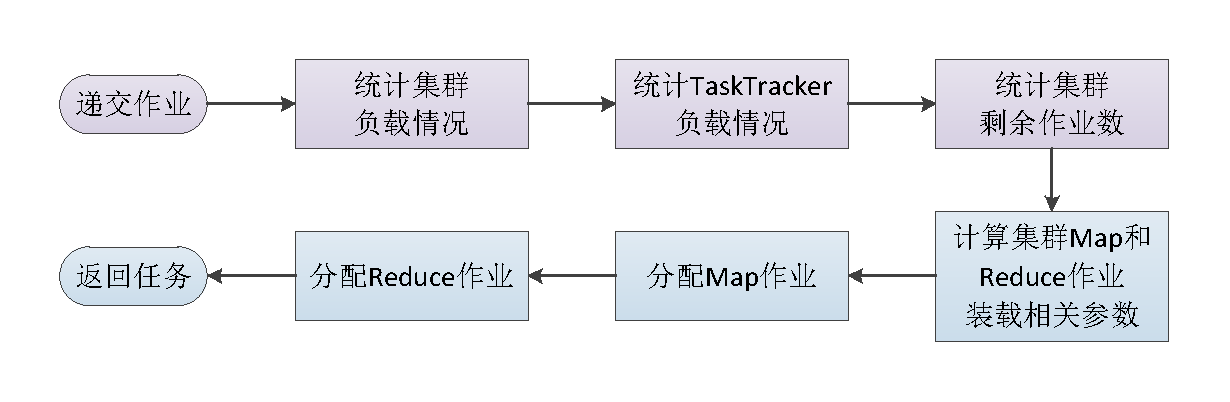
\includegraphics[width=1\textwidth]{调度器}
 \caption{调度器}
 \label{fig:调度器}
\end{figure}

对于JobQueueTaskScheduler的任务调度原则可总结如下:

\begin{enumerate}
\item 任务先进先出;
\item 尽量使集群每一个TaskTracker达到负载均衡(这个均衡是task数量上的而不是实际的工作强度);
\item 尽量分配作业的本地任务给TaskTracker,但不是尽快分配作业的本地任务给TaskTracker,最多分配一个非本地任务给TaskTracker(一是保证任务的并发性,二是避免有些TaskTracker的本地任务被偷走),最多分配一个reduce任务;
\item 为紧急的Task预留一定的slot;
\end{enumerate}

这种调度方式简单明了,JobTracker负载较小,适用于大多数的应用场景。

它的主要缺点就是对于在集群比较繁忙的情况,低优先级的作业将很难分配到集群的计算资源,这样对于那些低优先级同时又要求一定的响应时间的短作业来说是非常不利的。

为了解决这种应用差异性带来的性能损失,Hadoop允许用户自定义调度器。Hadoop的调度器被设计为一个可插拔的模块,用户可以根据自己实际应用要求设计调度器。

但由于调度机制在单机为分布式下的执行过于简单,其调度结果不具有参考价值,故在本文中不予以进一步的讨论。

\section{Hadoop运行机制对MapReduce性能的影响}
\subsection{原生Java}
通过第三章的测试结果可以看出,原生Java程序运行时,Map在经过一次大量的读操作之后,其写操作和Reduce的读写操作均经过合并优化。Map的结果被很好的合并,并交给了Reducer进行处理。程序运行效率非常高。

由于Hadoop提供了类库,所有操作均可通过接口实现,且对Hadoop内部透明,方便数据合并及优化,降低了I/O压力,性能损失很小。

\subsection{基于Streaming的实现}
通过第三章的的测试结果可以看出,基于Streaming的实现,Python的运行时间随着文件的增大逐渐比Java长,性能变差的主要是因为Map的结果没有进行combine。从表可以看出,Streaming中的Map和Reduce结果没有经过任何Combine,直接存入本地磁盘,从而造成了大量的空间浪费,增大了I/O负担,进入Reduce进一步处理的数据没有经过合并,造成性能损失。

以处理1亿条日志为例,从表可以得出,Streaming的实现与Java相比,写入量增大约100倍,读入量增大约10万倍,内存使用量增大约3倍,Reduce函数输入量增大了约15万倍,造成了性能损失。

由此可见,MapReduce框架中的输入输出优化、缓存和合并机制是MapReduce程序运行效率的关键。

\section{节点计算能力对MapReduce性能的影响}
Hadoop中,作业在TaskTracker上执行,TaskTracker的计算能力直接影响着Hadoop的整体性能。MapReduce是分布式计算框架,节点之间的通信通过网络传输。在Map和Reduce过程中,Hadoop产生了大量的网络和磁盘I/O,尤其是在Mapper和Reducer结束时,会引起数据量极大的“网络风暴”,这在实际生产环境中会给网卡和交换机带来很大的压力,若配置不当,将会成为MapReduce的瓶颈。

同时,在Hadoop运行过程中,Reduce在shuffle阶段对下载来的Map数据,并不是立刻就写入磁盘的,而是会先缓存在内存中,然后当使用内存达到一定量的时候才刷入磁盘,这就要求节点机有足够大的内存去缓存数据,默认情况下,reduce会使用其heapsize的70\%来在内存中缓存数据。内存的大小决定了缓存数量的多少,减少不必要的I/O。

磁盘读写速度也是MapReduce中影响性能的一个重要指标,在Map阶段,Hadoop会将Map的中间结果保存在节点本地磁盘,因为中间结果是临时的,不需要写多份。本地磁盘的读写I/O速度在某些应用中也会成为MapReduce程序的瓶颈。

另外,在实际生产环境中,节点计算之间的计算能力会有略微的不同,默认的Hadoop调度器会使作业运行时出现性能短板,这种短板在异构环境中尤为明显。

\section{实例程序编写方法对MapReduce性能的影响}
通过Java和Streaming两种实现方式的比较,可以看出影响MapReduce较大的部分为Suffle部分,从MapReduce运行原理可以看出,Suffle部分的合并是根据Key值合并的,如何合理的选择Key值,降低Reducer的处理时间,对MapReduce程序的运行起着至关重要的作用。

但实际开发中,Key的分布并不一定是均匀的,极端情况下,所有数据共享一个Key,后果是reduce任务只会在集群其中一个节点上运行,不仅没有利用好集群处理能力,反倒因为大量数据集中而导致计算效率低下,降低程序整体运行效率。

作为了解决这个问题,程序员需要在编程时尽量选择分布均匀的参数作为Key,或者使用其他方法将Key打散。下文以Web日志处理中的处理UV为例,描述了一种打散Key的方法。

UV是独立访客 (unique visitor)的缩写,对于网站的用户粘度和回头率统计有着至关重要的作用。

在网站设计中,通常会给Cookie一个Key为uid,Value为用户id的一组数据。在Web日志中,该uid即可用来统计UV。

在未打散Key的情况下,uid的值会比较分散,但对于游客用户来说,uid值为空,即0,这就会造成Map的结果中,uid分布不均匀。这时,将uid的值设为用户ip的后三位,从而使游客的统计均匀的分发到不同的Key中。但仅仅这样做是不够的,每个uid都不同,会导致Map结果中Key的数量过多,不便于数据合并和传输。这时,可以使用取模函数对uid取模,将Key的数量控制在合适的范围之内。进而分发到不同的Reduce节点上。

在Reduce阶段,Reducer接收到Key/Value对时,可以对Cookie值进行判断,若uid为空,则访客数+1,反之则该uid的统计数+1。

具体实现流程如下图:

实际生产环境中,Key的打散和控制还有其他多种方法,如将字符串转换为整形数字提高处理速度、或者将一个MapReduce操作划分成两份MapReduce程序去执行。具体使用方法应该根据应用程序的要求来确定,在此不一一赘述。

\section{本章小结}
本章通过分析Hadoop运行过程和运行机制,结合第\ref{chap:3}章中的测试结果,
    \chapter{总结与展望}
\label{chap:5}

\section{本文总结}
本文通过对基于Hadoop实现的MapReduce编程框架的介绍,详述了MapReduce编程思想及Hadoop的实现过程,并在此基础上使用两种实现方式实现了Web访问日志程序的编写与其性能分析。

根据第三章的测试和第四章的分析,可以得出以下四个结论:

\begin{enumerate}
\item MapReduce运行效率高,分布式程序编写简单,是个优秀的编程框架。
\item I/O可能会造成MapReduce性能瓶颈
\item 现阶段,原生Java比Streaming效率高
\item MapReduce程序编写中,Key的选择对数据合并、Reduce分发有着至关重要的作用。
\end{enumerate}

\section{进一步的工作}



\begin{enumerate}
\item 使用不同的Hadoop调度机制,测试其对集群的影响,找出并总结其调度方式所对应的应用场景。
\item 找出Streaming中负责数据合并的部分,理解其处理过程并进行适当优化。
\end{enumerate}



%%----------------- 附件部分 ----------------- %%
%    \backmatter
    \begin{thanks}


\vskip 18pt


\end{thanks}

    \fontsize{10.5pt}{10.5pt}\selectfont
\begin{thebibliography}{10}

\bibitem{paper:Google-MapReduce}
Jeffrey Dean and Sanjay Ghemawat.
\newblock MapReduce: Simplified Data Processing on Large Clusters.
\newblock In OSDI, 2004

\bibitem{site:Hadoop}
Hadoop Project.
\newblock http://hadoop.apache.org/

\bibitem{site:Yahoo}
Yahoo! Launches World’s Largest Hadoop Production Application, Yahoo! Developer Network.
\newblock http://developer.yahoo.com/blogs/hadoop/2008/02/yahoo-worldslargest-production-hadoop.html


\bibitem{paper:Hadoop-Performance-in-Heterogeneous}
Matei Zaharia, Andy Konwinski, Anthony D. Joseph, Randy Katz, Ion Stoica.
\newblock Improving MapReduce Performance in HeterogeneousEnvironments.
\newblock IN OSDI, 2008.8


\bibitem{book:Hadoop}
Tom White.
\newblock Hadoop: The Definitive Guide.
\newblock Yahoo Press; Second Edition edition (October 12, 2010)

\bibitem{site:hdfs}
Hadoop Distributed File System.
\newblock http://hadoop.apache.org/hdfs/

\bibitem{site:hadoop-counter}
MapReduce:默认Counter的含义.
\newblock http://langyu.iteye.com/blog/1171091

\bibitem{site:weblog}
WEB日志格式.
\newblock http://webdataanalysis.net/reference-and-source/weblog-format/

\bibitem{site:nginx}
Nginx.
\newblock http://www.nginx.org/

\bibitem{site:netcraft_nginx}
May 2012 Web Server Survey.
\newblock http://news.netcraft.com/archives/2012/05/02/may-2012-web-server-survey.html


\bibitem{paper:A-Dynamic-MapReduce-Scheduler-for-Heterogeneous-Workloads}
Chao Tian, Haojie Zhou,Yongqiang He, Li Zha.
\newblock A Dynamic MapReduce Scheduler for Heterogeneous Workloads
\newblock in Proceedings of the 2009 Eighth International Conference on Grid and Cooperative Computing, ser. GCC ’09. Washington, DC, USA: IEEE Computer Society, 2009, pp.218–224

% other

\bibitem{paper:Apache-Hadoop-Performance-Tuning-Methodologies-and-Best-Practices}
Shrinivas B. Joshi.
\newblock Apache Hadoop Performance-Tuning Methodologies and Best Practices
\newblock in Proceedings of the 2009 Eighth International Conference on Grid and Cooperative Computing, ser. GCC ’09. Washington, DC, USA: IEEE Computer Society, 2009, pp.241-242 

\bibitem{site:hadoop-wiki}
Hadoop Wiki.
\newblock http://wiki.apache.org/hadoop/

\bibitem{book:java}
Bruce Eckel、陈昊鹏.
\newblock Java编程思想(第4版).
\newblock 机械工业出版社

\bibitem{book:python}
Magnus Lie Hetland、司维等.
\newblock Python基础教程(第2版).
\newblock 人民邮电出版社

\bibitem{book:linux}
鸟哥、王世江.
\newblock 鸟哥的Linux私房菜:基础学习篇(第三版).
\newblock 人民邮电出版社

\end{thebibliography}


%%----------------- 附录部分 ----------------- %%
    \appendix
	\pagestyle{content}
    \chapter[实验环境搭建]{实验环境搭建}
\label{chap:fuluA}
Hadoop使用Java语言实现,集群之间以ssh协议通信,故Hadoop的依赖较少,且安装较为简便,其大体过程为:安装操作系统,安装ssh和jdk,解压缩Hadoop二进制包,编辑Hadoop配置文件并设置ssh、jdk和hadoop环境变量。
本文以具体过程如下:

1.最小化安装centos\_6.2\_x86-64

2.设置网络,并将源设置为西电源,关闭防火墙

\begin{verbatim}
iptables -F
iptables -X
iptables -Z
iptables-save > /etc/sysconfig/iptables
\end{verbatim}
3.更新系统

\begin{verbatim}
yum upgrade –y
\end{verbatim}
4.安装依赖包rsync openssh-server openssh-clients

\begin{verbatim}
yum install -y rsync openssh-server openssh-clients
\end{verbatim}
5.下载sun-jdk和hadoop包
6.安装jdk到/usr/lib并创建相应软链接

\begin{verbatim}
cp jdk-6u31-linux-x64.bin /usr/lib
cd /usr/lib
sh jdk-6u31-linux-x64.bin
rm jdk-6u31-linux-x64.bin
ln -s jdk1.6.0_31 jdk
\end{verbatim}
7.创建hadoop用户和用户组,并设置密码

\begin{verbatim}
groupadd hadoop
useradd -g hadoop hadoop –d /home/hadoop
passwd hadoop
\end{verbatim}
8.创建ssh密钥公钥,并加入可信列表

\begin{verbatim}
su hadoop
ssh-keygen -t rsa -P ""
cat ~/.ssh/id_rsa.pub >> ~/.ssh/authorized_keys
\end{verbatim}
验证密钥登录是否生效

\begin{verbatim}
ssh localhost
\end{verbatim}
若没生效,检查文件权限

\begin{verbatim}
chmod 644 ~/.ssh/authorized_keys
\end{verbatim}
9.解压缩hadoop-1.0.1到/usr/local并创建软链接

\begin{verbatim}
su
cp hadoop-1.0.1.tar.gz /usr/local
cd /usr/local
tar zxvf hadoop-1.0.1.tar.gz
ln -s hadoop-1.0.1 hadoop
chown hadoop:hadoop hadoop-1.0.1 hadoop -R
\end{verbatim}
10.给hadoop用户设置环境变量

\begin{verbatim}
vi ~/.bashrc
\end{verbatim}
文件末尾添加环境变量如下:

\begin{verbatim}
# Set Hadoop-related environment variables
export HADOOP_HOME=/usr/local/hadoop
# Set JAVA_HOME (we will also configure JAVA_HOME directly for Hadoop later on)
export JAVA_HOME=/usr/lib/jdk
# Add Hadoop bin/ directory to PATH
export PATH=$PATH:$HADOOP_HOME/bin
\end{verbatim}
重新登录使变量生效
11.编辑hadoop配置(/usr/local/hadoop/conf)

\begin{verbatim}
conf/hadoop-env.sh
\end{verbatim}
替换

\begin{verbatim}
# export JAVA_HOME=/usr/lib/j2sdk1.5-sun
\end{verbatim}
为

\begin{verbatim}
export JAVA_HOME=/usr/lib/jdk
\end{verbatim}
添加

\begin{verbatim}
# Disable the HADOOP_HOME_WARN
export HADOOP_HOME_WARN_SUPPRESS=TRUE
\end{verbatim}
取消hadoophome设置警报
core-site.xml 

\begin{verbatim}
<configuration>
     <property>
         <name>fs.default.name</name>
         <value>hdfs://localhost:9000</value>
     </property>
</configuration>
\end{verbatim}
hdfs-site.xml 

\begin{verbatim}
<configuration>
     <property>
         <name>dfs.replication</name>
         <value>1</value>
     </property>
</configuration>
\end{verbatim}
mapred-site.xml 

\begin{verbatim}
<configuration>
     <property>
         <name>mapred.job.tracker</name>
         <value>localhost:9001</value>
     </property>
</configuration>
\end{verbatim}
12.格式化hdfs

\begin{verbatim}
hadoop namenode -format
\end{verbatim}
13.启动hadoop

\begin{verbatim}
start-all.sh
\end{verbatim}
运行命令jps,查看Hadoop进程启动情况。如果
TaskTracker、DataNode、Jps、NameNode、SecondaryNameNode和JobTracker子进程均成功启动,则Hadoop运行正常。
至此,Hadoop就安装完成了。





\end{document}